{
{\sffamily I dette afsnit præsenterer vi vores resultater fra
eksperimentet, hvor vi har brugt den udvidede metode, til at vurdere
regionerne. Da eksperimentet blev kørt, satte vi opløsningen, på
regionernes approksimation med et gitter, for højt, hvilket resulterede
i, at kørslen ikke fik analyseret hele vores datasæt på grund af
tidsmangel.
}

\subsection{Reduceret datasæt}
Kørslen har nået at analysere $608$ malerier, men som vist herunder i
tabel \ref{ud_tabel_fjern_detaljer}, har vi kun $524$ brugbare
resultater, når vi har fjernet de billeder, som ikke er hele malerier.
Dette svarer til en nedgang på $13.82\%$.

\begin{table}[H]
    \centering
    \begin{tabular}{r@{\ \ }p{12em}r|r@{.}l}
            & Analyserede malerier & $608$ & $100$ & $00\%$   \\
        $-$ & Udsnit af malerier   &  $84$ &  $13$ & $82\%$   \\\hline
            & Resultater           & $524$ &  $86$ & $18\%$
    \end{tabular}
    \caption[]{Udregning af brugbare resultater fra udvidet kørsel.}
    \label{ud_tabel_fjern_detaljer}
\end{table}

Dette svarer til $3.65\%$ af de brugbare resultater fra den
naive kørsel. Vores datasæt bliver gennemgået alfabetisk efter
kunstnerens efternavn, så vi har kun resultater fra kunstnere med
efternavn startende med 'A' og 'B'.

At vi kun har et undersæt af malerierne gør, at vi bliver nødt til at se
på hvilke tidsperioder og nationaliteter vi har repræsenteret. Graferne
i figur \ref{ud_year_nation} viser at italienske kunstnere, er kraftigt
overrepræsenteret, og at malerierne primært er fra perioden 1401 --
1650. Dette er ikke overraskende, siden datasættet i forvejen
favoriserer denne type malerier.

\begin{figure}[!h]
    \centering
    \subfloat[Årstal]{
    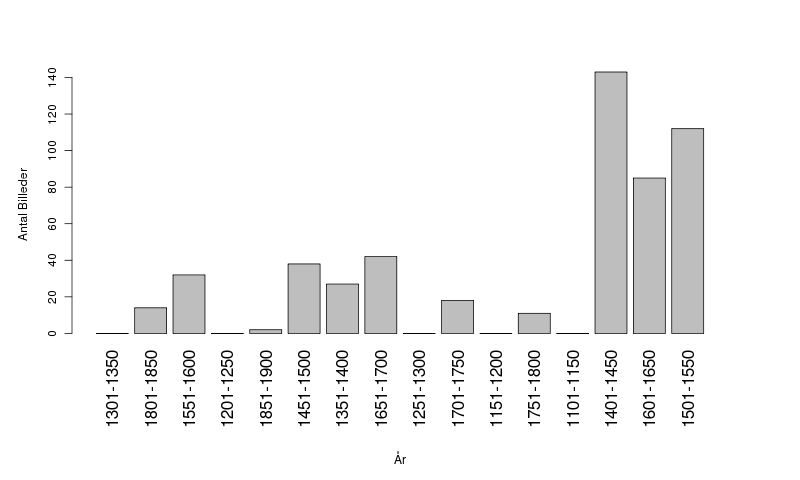
\includegraphics[angle=-90,width=0.42\textwidth]{afsnit/resultater/billeder/year}
        \label{ud_year}}\hspace{1em}
    \subfloat[Nationalitet]{
        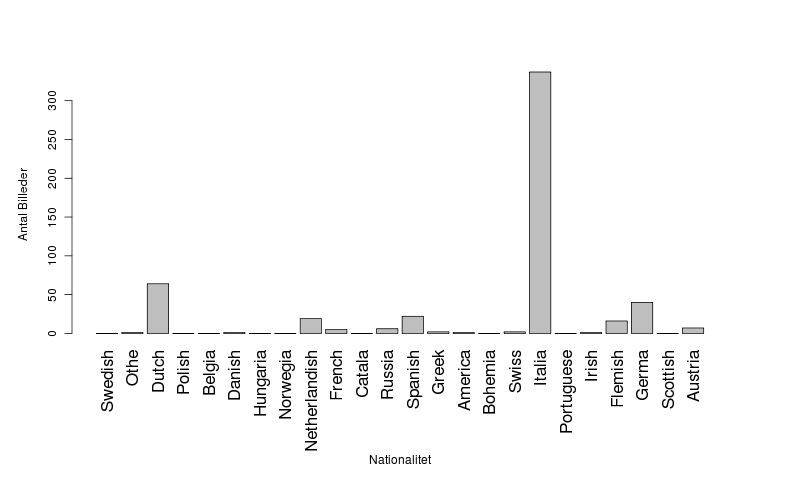
\includegraphics[angle=-90,width=0.42\textwidth]{afsnit/resultater/billeder/nation}
        \label{ud_nation}}
    \caption[]{Maleriernes årstal og nationalitet.}
    \label{ud_year_nation}
\end{figure}

\subsection{Håndtering af systematisk fejl}
Selvom denne analyse også har brugt den fejlbehæftede metode, til
udtrækning af regioner, så sorteres duplikater fra, når vi approksimerer
en region. Vi har gemt farven, som en region er blevet tildelt af
floodfill, og hvis denne farve ikke er at finde i regionens begrænsende
rektangel, betyder det, at regionen er blevet malet over senere. Vi
smider derfor denne region væk.

Den udvidede metode indeholder derfor ingen duplikater, men resultaterne
er ikke direkte sammenlignelige med dem fra den naive kørsel.

\subsection{Resultater}
Udregningen i tabel \ref{ud_tabel_fordeling} redegør for, hvor mange af
de brugbare resultater, der har mindst en region liggende i det gyldne
snit. Vi ser at der i $87.02\%$ af malerierne, er blevet fundet regioner
i det gyldne snit, og vi kan derfor ikke afvise hypotese
\ref{hypo_binaer}.

\begin{table}[H]
    \centering
    \begin{tabular}{r@{\ \ }p{12em}r|r@{.}l}
            & Positive resultater   & $456$ &  $87$ & $02\%$ \\
        $+$ & Negative resultater   &  $68$ &  $12$ & $98\%$ \\\hline
            & Resultater i alt      & $524$ & $100$ & $00\%$
    \end{tabular}
    \caption[]{Et positivt resultat beskriver et maleri hvori der er
    fundet mindst en region i det gyldne snit, ved brug af den udvidede
    vurdering af regioner. Over halvdelen af malerierne har således
    mindst en region i det gyldne snit.}
    \label{ud_tabel_fordeling}
\end{table}

Fordelingen af regioner, over de fire gyldne snit i malerierne, ses i
tabel \ref{ud_tabel_fire_snit}. Ved at undersøge afvigelsen mellem
ekstremerne i snit 0 og 2, ser vi at disse afviger med $(499 -
405)/405 = 0.2320988 = 23.2 \%$ fra hinanden, og vi kan således afvise
hypotese \ref{hypo_fire_g_snit}.

\begin{table}[H]
    \centering
    \begin{tabular}{r@{\ \ }p{12em}r}
            & Regioner i $GS$ 0         &  $405$ \\
        $+$ & Regioner i $GS$ 1         &  $421$ \\
        $+$ & Regioner i $GS$ 2         &  $499$ \\
        $+$ & Regioner i $GS$ 3         &  $492$ \\\hline
            & Regioner i de fire $GS$   & $1817$
    \end{tabular}
    \caption[]{Forholdet mellem de interessante regioner fundet i de
    fire gyldne snit ved udvidet vurdering. Der er afvigelse, mellem
    ekstremerne, på $23.2 \%$. Ligesom i den naive kørsel, er det
    nederste horisontale snit det mest brugte.}
    \label{ud_tabel_fire_snit}
\end{table}


I figur \ref{antal_regioner_vertikale_cut_udvidet} er det samlede antal
fundne regioner, i de 20 vertikale snit, for hele datasættet,
afbilledet. Det ses at der er fundet markant flere regioner, i de to snit som
ligger tættest på miden, og færrest ud i kanterne.

\begin{figure}[h!]
	\begin{center}
		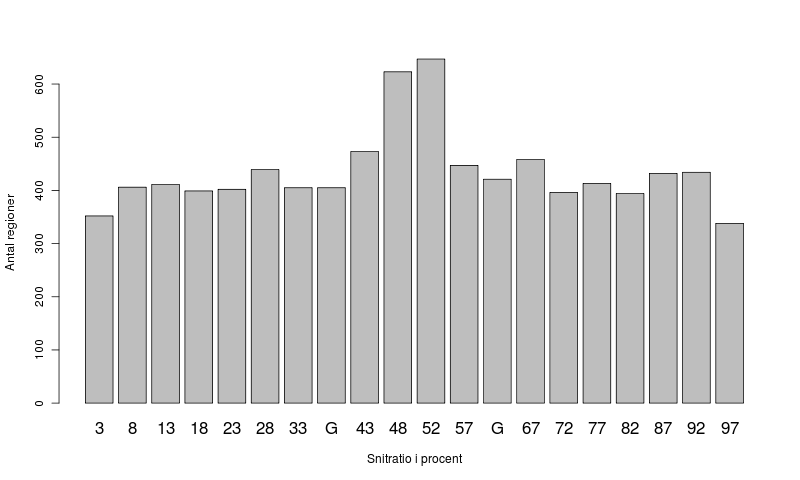
\includegraphics[width=0.9\textwidth]{afsnit/resultater/billeder/cut0cut1eatsperratioU.png}
	\end{center}
	\caption{Antal regioner i hvert af de 20 vertikale snit}
	\label{antal_regioner_vertikale_cut_udvidet}
\end{figure}

I figur \ref{antal_regioner_horisontale_cut_udvidet} er samme afbildning
lavet for det horisontale plan, hvor venstre side af grafen svarer til
toppen af billedet. I denne graf er det snitratioerne $72$ og $82$ som
har flest fundne regioner. Fra snitratio $52$ og ned, falder antal
regioner gradvist. Fra snitratio $52$ og op, svinger antallet af
regioner. Kanterne er igen klart de laveste i grafen.

\begin{figure}[h!]
	\begin{center}
		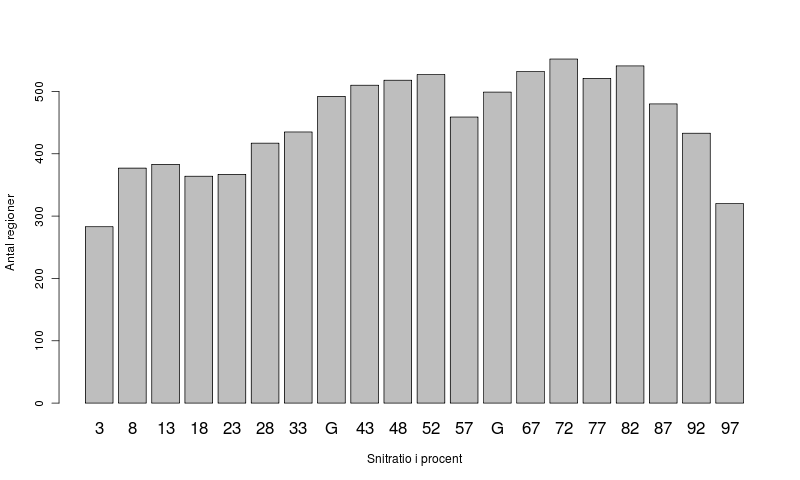
\includegraphics[width=0.9\textwidth]{afsnit/resultater/billeder/cut2cut3eatsperratioU.png}
	\end{center}
    \caption{Antal regioner i hvert af de 20 horisontale snit, hvor
    venstre side af grafen repræsenterer øverste del af malerierne.}
    \label{antal_regioner_horisontale_cut_udvidet}
\end{figure}

Ud fra disse observationer kan vi konkludere at der ikke er flere
regioner i det gyldne snit, end i midten af malerierne, og vi kan derfor
forkaste hypotese \ref{hypo_alle_andre_snit} og \ref{hypo_midten}.

I figur \ref{G_vs_to_trejedele_udvidet}, er de fire gyldne snit, samt
$\frac{2}{3}$ repræsenteret. Det ses at der ikke er nogen entydighed på
hvilken ratio, som er dominerende, og vi kan derfor forkaste hypotese
\ref{hypo_to_tredjedele}.

Figur \ref{G_vs_to_trejedele_udvidet} viser også, at antallet af fundne
regioner i det gyldne snit og snitratioen $\frac{2}{3}$, ligger meget
tæt på hinanden, og den største forskel ligger ikke på mere end $15\%$.
Vi kan derfor ikke afvise hypotese \ref{hypo_15p}.

\begin{figure}[h!]
	\begin{center}
		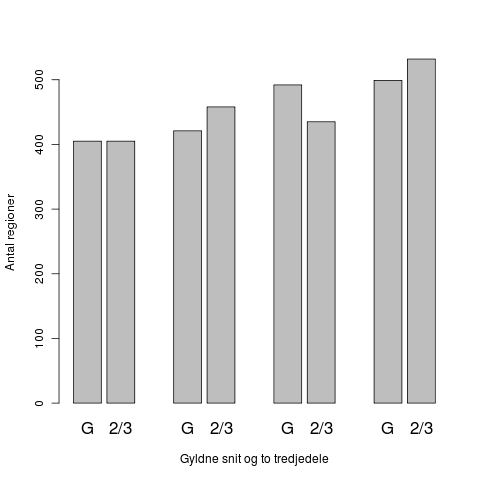
\includegraphics[width=0.6\textwidth]{afsnit/resultater/billeder/G_vs_to_tredjedeleU.png}
	\end{center}
	\caption{Procentvis antal regioner i de fire gyldne snit og deres
    tilhørende $\frac{2}{3}$-snit.}
	\label{G_vs_to_trejedele_udvidet}
\end{figure}

I graferne i figur \ref{udvidet_year}, kan man se hvor mange regioner
der er fundet i gennemsnit per billedet i alle tidsperioder.
Tidsperioder, hvor ingen malerier er analyseret, er ikke taget med. Det
ses at i tidsperioden 1401 -- 1450, findes mange flere end de andre
tidsperioder, og i visse tilfælde doubbelt så mange. Da doubbelt så
mange regioner er skarpt større end $10\%$ afvigelse, kan vi forkaste
hypotese \ref{hypo_tid}.

\begin{figure}[!h]
	\begin{center}
		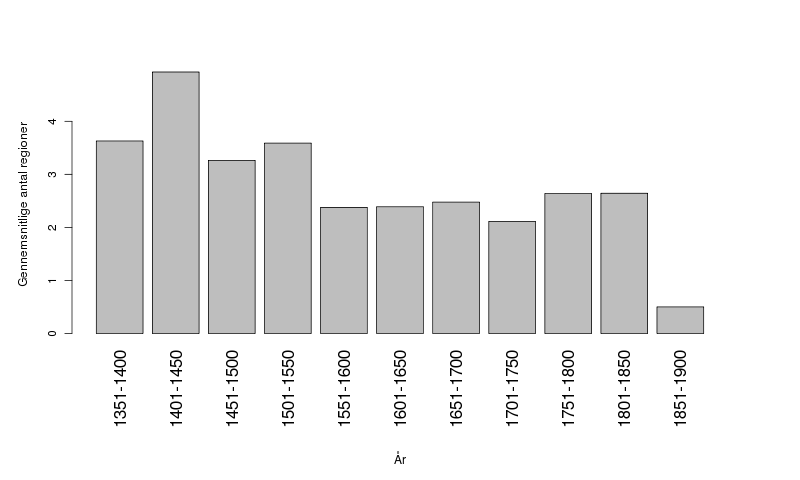
\includegraphics[angle=0,width=0.90\textwidth]{afsnit/resultater/billeder/yearcutU.png}
	\end{center}
    \caption{Graf over det gennemsnitlige antal regioner fundet i hver
    tidsperiode. Hver graf repræsenterer hvert deres snit.}
	\label{udvidet_year}
\end{figure}

I graferne i figur \ref{udvidet_nation}, ses at det er meget svingene
fra hvilke nationer, billeder med mange regioner i det gyldne snit,
kommer fra. Holland ligger sig lidt foran de andre. Danmark har slet
ikke nogle malerier hvor der er fundet regioner i det gyldne snit. Alle
nationer, hvor analysen ikke har bearbejdet nogle malerier, er sorteret
fra. Da malerier fra Holland har flere end $10\%$ højre gennemsnitlige
fundne regioner, end Danmark og Frankrig, holder hypotese
\ref{hypo_nation} ikke, og kan derfor forkastes.

\begin{figure}[!h]
	\begin{center}
		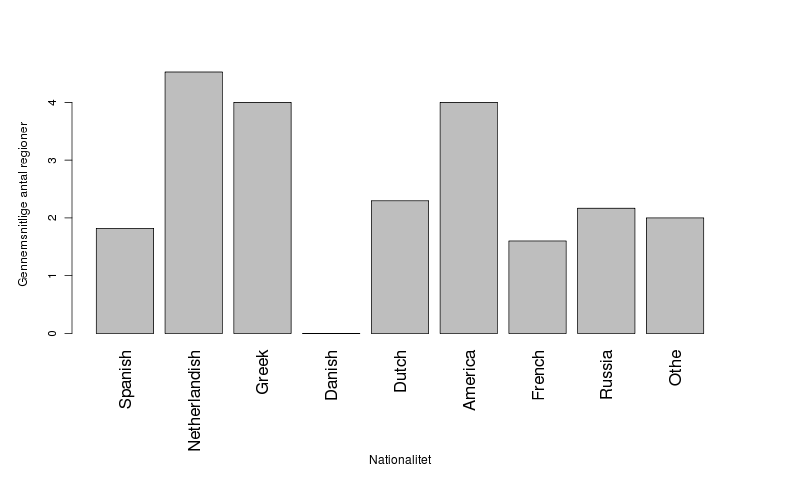
\includegraphics[angle=0,width=0.90\textwidth]{afsnit/resultater/billeder/nationcutU.png}
	\end{center}
    \caption{Graf over gennemsnitligt antal fundne regioner i det gyldne
    snit fra hver nationalitet.}
	\label{udvidet_nation}
\end{figure}

\subsubsection{Antallet af fundne regioner over alle snit}
Analysen har fundet $17,705$ regioner over alle snit i malerierne, med
middelværdi $\mu = 33.79$ og standardafgivelse $\sigma = 18.58$.
Antallet af fundne regioner i malerierne er illustreret i figur
\ref{ud_graf_total_regions}. I figur \ref{ud_qq_total_regions} er vist
et QQ-plot, som viser hvorvidt vores data er normalfordelt. Dette er
tilfældet, hvis punkterne følger diagonalen i grafen. Vi ser, at de
observerede data følger linjen nogenlunde, men har et udsving nederst
til venstre, hvilket antyder at fordelingen er lidt skæv. Vi har i figur
\ref{ud_hist_total_regions} sammenlignet et histogram over de
observerede værdier, med tæthedsfunktionen for normalfordelingen $X \sim
N(\mu = 33.79, \sigma^2 = 345.22)$. De observerede værdier, følger dog
ikke de teoretiske værdier særlig pænt, og kun få steder falder de
teoretiske værdier inden for det observerede interval, hvorfor vi ikke
kan komme frem til et troværdigt konfidensinterval.

Med et større antal fundne regioner, kunne vi meget vel komme tættere på
en normalfordeling, og vi kunne da udtale os mere sikkert, om det
forventede antal fundne regioner i et arbitrært billede.

\begin{figure}[!h]
    \centering
    \subfloat[]{
        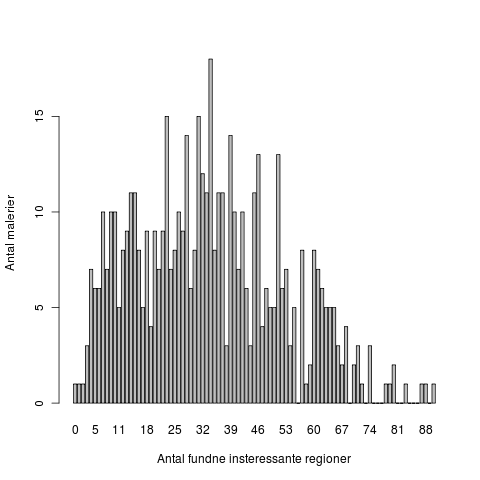
\includegraphics[width=0.49\textwidth]{afsnit/resultater/billeder/exp_totalregions}
        \label{ud_graf_total_regions}
    }
    \subfloat[]{
        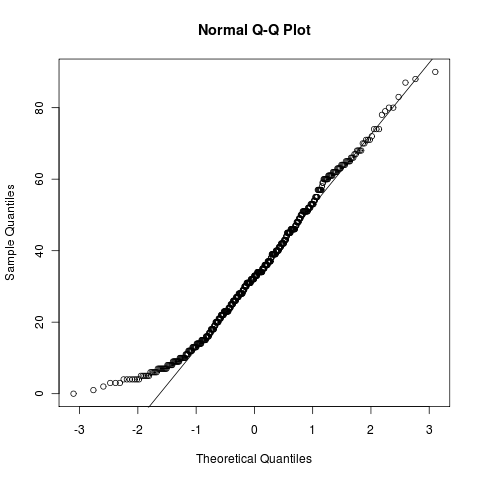
\includegraphics[width=0.49\textwidth]{afsnit/resultater/billeder/qq_exp_totalregions}
        \label{ud_qq_total_regions}
    }\\
    \subfloat[]{
        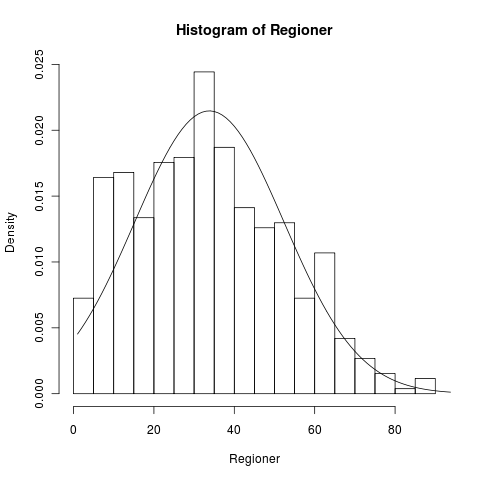
\includegraphics[width=0.62\textwidth]{afsnit/resultater/billeder/hist_exp_totalregions}
        \label{ud_hist_total_regions}
    }
    \caption[]{Fordelingen af fundne regioner på malerier ved udvidet
    vurdering.
    \textbf{\ref{ud_graf_total_regions}:} Fordelingen af de fundne
    regioner.
    \textbf{\ref{ud_qq_total_regions}:} QQ-plot, som viser at vi er tæt
    på at have en normalfordeling med den teoretiske fordeling $X \sim N(\mu,
    \sigma^2)$.
    \textbf{\ref{ud_hist_total_regions}:} Histrogram med
    tæthedsfunktionen for normalfordeling, hvor $\mu = 33.79$ og
    $\sigma^2 = 345.22$.
    }
    \label{ud_total_regions_plots}
\end{figure}

\subsection{Opsamling}
Vi vil nu samle op på de ovenstående resultater for vores eksperiment
med udvidet vurdering af interessante regioner. Tabel \ref{hypoteser_udvidet} viser
hvordan vores resultater forholder sig til vores opstillede hypoteser.
Vi giver vores vurdering af, hvad resultaterne siger om brugen af det
gyldne snit, men vær opmærksom på, at vi ikke er fagfolk i
kunstforståelse og vores fortolkninger kun bygger på de observerede
resultater.

\begin{table}[!h]
    \centering
    \begin{tabular}{|c|l|c|c|}
        \hline
        \textbf{Hypotese nr.} & \textbf{Beskrivelse} & \textbf{Afvist} &
        \textbf{Ikke afvist}  \\\hline\hline
        1 & Mindst én region i $GS$                     &            & \checkmark   \\\hline
        2 & Alle fire $GS$ lige meget brugt             & \checkmark &              \\\hline
        3 & $1/3$ har lærred med forholdet $1:\varphi $ & \checkmark$^{\textrm{*}}$ &              \\\hline
        4 & Flest regioner i $GS$                       & \checkmark &              \\\hline
        5 & Flere regioner i $GS$ end $\frac{2}{3}$     & \checkmark &              \\\hline
        6 & Flere regioner i $GS$ end i midten          & \checkmark &              \\\hline
        7 & $GS$ brugt lige meget, uanset tidsperiode   & \checkmark &              \\\hline
        8 & $GS$ brugt lige meget, uanset nationalitet  & \checkmark &              \\\hline
        9 & $\frac{2}{3}$ brugt som approksimation til $GS$   &      & \checkmark	\\\hline
    \end{tabular}
    \caption[]{Hypoteser i forhold til den naive kørsel. $GS$ bruges som
    forkortelse for det gyldne snit.  $^{\textrm{*}}$Jvf. udregning
    \ref{tabel_real_dimensions} }
    \label{hypoteser_udvidet}
\end{table}

Hypotese 1 kan ikke afvises, hvilket betyder at over halvdelen af de
analyserede malerier, har mindst én interessant region i det gyldne
snit. Da vi mener at malerier konstrueret efter det gyldne snit, vil
have mindst én interessant region i det gyldne snit, kan vi ikke afvise
at det gyldne snit bliver brugt af kunstnere i malerier.

Vores resultater afviser hypotese 2, hvilket betyder, at antallet af
interessante regioner fundet i de enkelte gyldne snit afviger meget fra
hinanden.  Dette tyder på, at kunstnere favoriserer nogle gyldne snit
frem for andre. Når denne hypotese afvises, mener vi ikke, at det gyldne
snit kan tillægges nogen speciel æstetisk værdi: Tror man på, at det
gyldne snit er specielt æstetisk tiltalende, må \emph{alle} gyldne snit
være lige æstetisk tiltalende. Derfor må man jo netop forvente at finde
nogenlunde samme antal regioner i hvert snit.

Da hypotese 3 ikke bestemmes af, hvilken metode interessante regioner
bedømmes efter, har vi allerede afvist denne. Nærmere forklaring er
givet i afsnit \ref{naiv_opsamling} ved eksperimentet med naiv vurdering
af regioner.

Vi afviser hypotese 4, hvilket fortæller os, at der ikke er blevet
fundet flere interessante regioner i det gyldne snit, end i alle andre
snit.  I billeder komponeret efter det gyldne snit, må man forvente at
de interessante regioner koncentrerer sig om snittet. Vi mener derfor
ikke at det er retfærdigt at sige, at kunstnere arbejder ud fra det
gyldne snit, når et maleri komponeres.

Hypotese 5 afvises, fordi vi ikke kan finde flere interessante regioner
i det gyldne snit, end i snittet ved $\frac{2}{3}$, i alle fire snit. Vi
mener derfor, at dette er en indikation på, at kunstneren ikke er helt
bevidst om, hvor det gyldne snit ligger, hvis han da forsøger at male
efter dette.

Vi afviser hypotese 6, fordi vi finder flere interessante regioner i
midten af malerier, end i det gyldne snit. Vi mener derfor at der er
mere belæg for at vise, at kunstnere opbygger malerier ud fra midten,
end ud fra det gyldne snit.

Hypotese 7 afvises af grafen i figur \ref{udvidet_year}, fordi det
gennemsnitlige antal af interessante regioner mellem tidsperioder
afviger med mere end $10 \%$. Det er interessant at se på antallet af
regioner fundet i det gyldne omkring de historiske milestene. Det lader
til, at brugen af det gyldne snit falder efter 1550. I tidperioden 1851
-- 1900 har vi kun to malerier, hvilket kan være forklaringen på det
drastiske fald i antal fundne regioner.

Hypotese 8 bliver afvist, da det gennemsnitlige antal af fundne
interessante regioner i det gyldne snit afviger for meget mellem
nationaliteter. Vi mener, at dette indikerer at nogle nationer er mere
fascineret af det gyldne snit end andre.

Vi kan ikke afvise hypotese 9. Det betyder at antallet af interessante
regioner fundet i det gyldne snit, ikke afviger med mere end $15 \%$ fra
antallet fundet i snittet ved $\frac{2}{3}$. Dette kan tyde på, at
snittet ved $\frac{2}{3}$ bruges som en approksimation til det gyldne
snit. Dette passer også meget fint sammen med at hypotese 5 er blevet
afvist.

} % Eh eh eh. Nallerne væk!

% vim: set tw=72 spell spelllang=da:
